\chapter{Drucken der Abschlussarbeit}
\label{cha:Drucken}




\section{PDF-Workflow}
\label{sec:pdf}

In der aktuellen Version wird \latex\ so benutzt, dass damit direkt PDF-Dokumente (ohne den früher üblichen Umweg über DVI und PS) erzeugt werden.
Zur Arbeit mit dem Sumatra PDF-Viewer unter Windows und TeXnicCenter ist ein passendes Ausgabeprofil vorbereitet
(s.\ Abschn.\ \ref{sec:VerwendungUnterWindows} im Anhang).%



\begin{comment}

\section{DVI-PS-Workflow (optional)}

Dieser Abschnitt ist nur dann relevant, wenn \latex\ im ("alten") "Kompatibilitätsmodus" verwendet wird,
in dem die druckfähige PDF-Datei über DVI- und PostScript-Zwischendateien erzeugt wird. 
Dieser Modus ist weiterhin notwendig, wenn das \texttt{psfrag}-Package verwendet wird
(s.\ Abschnitt \ref{sec:psfrag}).

\subsection{DVI-Dateien}

\latex selbst erzeugt sogenannte DVI-Dateien (\emph{device independent}), die man mit einem
DVI-\emph{Viewer} wie
\zB\ \texttt{Yap}%
\footnote{\emph{Yet Another Previewer} von Christian Schenk, Teil der
MikTeX-Installation.}
betrachten und auch drucken kann. Falls das Dokument EPS-Grafiken
enthält, muss auch \emph{GhostScript} installiert sein, um Bilder und Grafiken im DVI-Previewer 
direkt betrachten zu können.%
\footnote{In den aktuellen MikTeX-Installationen ist eine spezielle Version von GhostScript (\texttt{mgs.exe}) für die interne Darstellung von Grafiken in YAP bereits enthalten.}



\subsection{PostScript- und PDF-Dateien}

PostScript-Dateien erzeugt man mit dem Programm \texttt{dvips}, das Teil der
\latex-Installation ist.
Die damit generierten Files sind vollständig, \dah sie enthalten auch die
vorgesehenen EPS-Grafiken, und sind daher in der Regel umfangreich.
Eine PS-Datei kann man entweder direkt betrachten (\zB mit \texttt{ghostview}%
\footnote{\url{www.gnu.org/software/ghostview/}}%
), drucken, oder mithilfe von \texttt{ps2pdf} (\bzw\ \texttt{gswin32c.exe} in der GhostScript-Installation unter Windows) in eine
PDF-Datei umwandeln (Abb.~\ref{fig:latex-pdf-workflow}):
%
\begin{center}
\begin{tabular}{lcl}
\texttt{latex da.tex}        & $\rightarrow$ & \texttt{da.dvi}\\
\texttt{dvips -ta4 -Ppdf da} & $\rightarrow$ & \texttt{da.ps}\\
\texttt{ps2pdf -sDEVICE=pdfwrite}  & $\rightarrow$ & \texttt{da.pdf}\\
%-sPAPERSIZE=a4 -dSAFER -dBATCH -dNOPAUSE -sDEVICE=pdfwrite -dPDFSETTINGS=/prepress -sOutputFile="%bm.pdf" -c save pop -f "%bm.ps"
\end{tabular}
\end{center}
In der \emph{TeXnicCenter}-Umgebung werden diese Schritte durch das Ausgabeprofil
\begin{center}
\verb!LaTeX => PS => PDF!
\end{center}
automatisch durchgeführt, wobei Adaptierungen der einzelnen Schritte durch Modifikation des entsprechenden Ausgabeprofils möglich sind. 
Zur Erzeugung einer hochqualitativen PDF-Datei ist für \texttt{ps2pdf} die zusätzliche Option \texttt{-dPDFSETTINGS=/prepress} zu empfehlen.
Weitere (aktuelle) Details zur Einstellung von Ausgabeprofilen unter TeXnicCenter und MikTeX finden sich in
Anhang \ref{sec:TeXnicCenterUndMikTeX}.



\begin{figure}
\centering
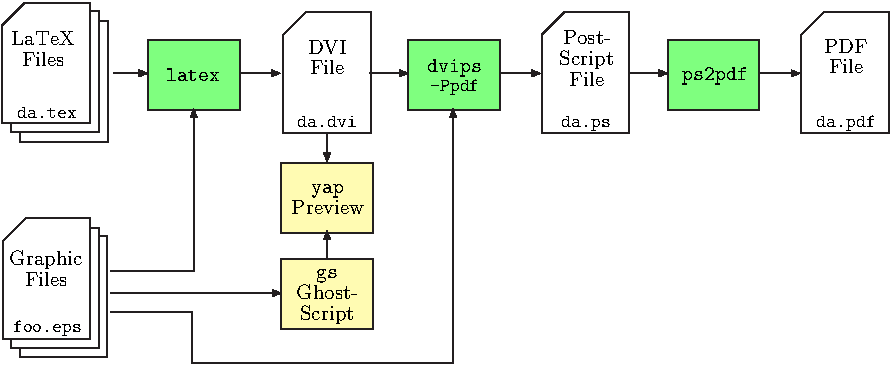
\includegraphics[width=1.0\textwidth]{workflow-cm}
\caption{Erzeugung von
PDF-Doku\-men\-ten im DVI-PS-Workflow. EPS-Grafiken werden erst bei der
Erzeugung der PS-Datei eingebunden. 
Anmerkung: Die abgebildete Vektorgrafik wurde mit \emph{Freehand} unter
Verwendung der \emph{BaKoMa} TrueType-Schriften erstellt %
(s.\ Abschn.\ \ref{sec:tex-schriften-in-grafiken}).}
\label{fig:latex-pdf-workflow}
\end{figure}

\end{comment}


\section{Drucken}

Vor dem Drucken der Arbeit empfiehlt es sich, einige Dinge zu beachten, um unnötigen Aufwand (und auch Kosten) zu vermeiden.

\subsection{Drucker und Papier}

Die Abschlussarbeit sollte in der Endfassung unbedingt auf einem
qualitativ hochwertigen Laserdrucker ausgedruckt werden, Ausdrucke
mit Tintenstrahldruckern sind \emph{nicht} ausreichend. Auch das
verwendete Papier sollte von guter Qualität (holzfrei) und
üblicher Stärke (mind.\ $80\; {\mathrm g} / {\mathrm m}^2$) sein.
Falls \emph{farbige} Seiten notwendig sind, sollte man diese einzeln%
\footnote{Tip: Mit \emph{Adobe Acrobat} lassen sich sehr einfach einzelne Seiten
des Dokuments für den Farbdruck auswählen und zusammenstellen.}
auf einem Farb-Laserdrucker ausdrucken und dem Dokument beifügen.

Übrigens sollten \emph{alle} abzugebenden Exemplare \textbf{gedruckt} (und nicht kopiert) werden! Die Kosten für den Druck
sind heute nicht höher als die für Kopien, der
Qualitätsunterschied ist jedoch -- \va\ bei Bildern und Grafiken
-- meist deutlich.


\subsection{Druckgröße}

Zunächst sollte sichergestellt werden, dass die in der fertigen PDF-Datei eingestellte
Papiergröße tatsächlich \textbf{A4} ist! Das geht \zB\ mit \emph{Adobe Acrobat}
oder \emph{SumatraPDF}
über \texttt{File} $\rightarrow$ \texttt{Properties},
wo die Papiergröße des Dokuments angezeigt wird:
\begin{center}
\textbf{Richtig:} A4 = $8{,}27 \times 11{,}69$ in \bzw\ $21{,}0 \times 29{,}7$ cm.
\end{center}
Falls das nicht stimmt, ist vermutlich irgendwo im Workflow versehentlich \textbf{Letter} 
als Papierformat eingestellt, %, häufig ist \emph{Adobe Distiller} "schuld".


Ein häufiger und leicht zu übersehender Fehler beim Ausdrucken von
PDF-Doku\-menten wird durch die versehentliche Einstellung der
Option "Fit to page" im Druckmenü verursacht, wobei die Seiten
meist zu klein ausgedruckt werden. Überprüfen Sie daher die Größe
des Ausdrucks anhand der eingestellten Zeilenlänge oder mithilfe
einer Messgrafik, wie am Ende dieses Dokuments gezeigt.
Sicherheitshalber sollte diese Messgrafik bis zur
Fertigstellung der Arbeit beibehalten und die entsprechende
Seite erst ganz am Schluss zu entfernt werden.
Wenn, wie häufig der Fall, einzelne Seiten getrennt in Farbe gedruckt 
werden, so sollten natürlich auch diese genau auf die Einhaltung der Druckgröße 
kontrolliert werden!




\section{Binden}

Die Endfassung der Abschlussarbeit%
\footnote{Für \textbf{Bachelorarbeiten} genügt, je nach Vorgaben des Studiengangs, meist eine einfache Bindung (Copyshop oder Bibliothek).}
ist in fest gebundener Form
einzureichen.%
\footnote{An der Fakultät Hagenberg ist bei Masterarbeiten zumindest eines der
Exemplare \emph{ungebunden} abzugeben -- dieses wird später von einem
Buchbinder in einheitlicher Form gebunden und verbleibt
danach in der Bibliothek. Datenträger sind bei diesem Exemplar lose 
und \emph{ohne} Aufkleber (jedoch beschriftet) beizulegen.}
Dabei ist eine Bindung zu
verwenden, die das Ausfallen von einzelnen Seiten nachhaltig
verhindert, \zB durch eine traditionelle Rückenbindung
(Buchbinder) oder durch handelsübliche Klammerungen aus Kunststoff
oder Metall. Eine einfache Leimbindung ohne Verstärkung ist
jedenfalls \emph{nicht} ausreichend.


Falls man -- was sehr zu empfehlen ist -- die Arbeit bei einem
professionellen Buchbinder durchführen lässt, sollte man auch auf
die Prägung am Buchrücken achten, die kaum zusätzliche Kosten
verursacht. Üblich ist dabei die Angabe des Familiennamens des
Autors und des Titels der Arbeit. Ist der Titel der Arbeit zu
lang, muss man notfalls eine gekürzte  Version angeben, wie \zB:
%
\begin{center}
\setlength{\fboxsep}{3mm}
\fbox{
\textsc{Schlaumeier}
\textperiodcentered\ \textsc{Part.\ Lösungen zur allg.\ Problematik}}
\end{center}
%



\section{Elektronische Datenträger (CD-R, DVD, USB-Stick)}
Speziell bei Arbeiten im Bereich der Informationstechnik (aber
nicht nur dort) fallen fast immer Informationen an, wie Programme,
Daten, Grafiken, Kopien von Internetseiten \usw, die für eine
spätere Verwendung elektronisch verfügbar sein sollten.
Vernünftigerweise wird man diese Daten während der Arbeit bereits
gezielt sammeln und der fertigen Arbeit auf einer CD-ROM, DVD oder
einem USB-Stick beilegen. Es ist außerdem sinnvoll -- schon allein
aus Gründen der elektronischen Archivierbarkeit -- die eigene Arbeit
selbst als PDF-Datei beizulegen.%
\footnote{Auch Bilder und Grafiken könnten in elektronischer Form nützlich
sein, die \latex- oder Word-Dateien sind hingegen überflüssig.}


Falls ein elektronischer Datenträger (CD-ROM, DVD, USB-Stick) beigelegt
wird, sollte auf folgende Dinge geachtet werden:
%
\begin{enumerate}
\item Jedem abzugebenden Exemplar muss eine identische Kopie des
Datenträgers beiliegen. %
\item Verwenden Sie qualitativ hochwertige Rohlinge und überprüfen
Sie nach der Fertigstellung die tatsächlich gespeicherten Inhalte
des Datenträgers! %
\item Der Datenträger sollte in eine im hinteren Umschlag
eingeklebte Hülle eingefügt sein und sollte so zu entnehmen sein,
dass die Hülle dabei \emph{nicht} zerstört wird (die
meisten Buchbinder haben geeignete Hüllen parat). %
\item Der Datenträger muss so beschriftet sein, dass er der
Abschlussarbeit eindeutig zuzuordnen ist, am Besten durch ein
gedrucktes Label%
\footnote{Nicht beim lose abgegebenen Bibliotheksexemplar --
dieses erhält ein standardisiertes Label durch die Bibliothek.} %
oder sonst durch \emph{saubere}
Beschriftung mit
der Hand und einem feinen, wasserfesten Stift. %
\item Nützlich ist auch ein (grobes) Verzeichnis der Inhalte des
Datenträgers (wie exemplarisch in Anhang \ref{app:materials}).
\end{enumerate}
